\documentclass{article}\usepackage[]{graphicx}\usepackage[]{color}
%% maxwidth is the original width if it is less than linewidth
%% otherwise use linewidth (to make sure the graphics do not exceed the margin)
\makeatletter
\def\maxwidth{ %
  \ifdim\Gin@nat@width>\linewidth
    \linewidth
  \else
    \Gin@nat@width
  \fi
}
\makeatother

\definecolor{fgcolor}{rgb}{0.345, 0.345, 0.345}
\newcommand{\hlnum}[1]{\textcolor[rgb]{0.686,0.059,0.569}{#1}}%
\newcommand{\hlstr}[1]{\textcolor[rgb]{0.192,0.494,0.8}{#1}}%
\newcommand{\hlcom}[1]{\textcolor[rgb]{0.678,0.584,0.686}{\textit{#1}}}%
\newcommand{\hlopt}[1]{\textcolor[rgb]{0,0,0}{#1}}%
\newcommand{\hlstd}[1]{\textcolor[rgb]{0.345,0.345,0.345}{#1}}%
\newcommand{\hlkwa}[1]{\textcolor[rgb]{0.161,0.373,0.58}{\textbf{#1}}}%
\newcommand{\hlkwb}[1]{\textcolor[rgb]{0.69,0.353,0.396}{#1}}%
\newcommand{\hlkwc}[1]{\textcolor[rgb]{0.333,0.667,0.333}{#1}}%
\newcommand{\hlkwd}[1]{\textcolor[rgb]{0.737,0.353,0.396}{\textbf{#1}}}%
\let\hlipl\hlkwb

\usepackage{framed}
\makeatletter
\newenvironment{kframe}{%
 \def\at@end@of@kframe{}%
 \ifinner\ifhmode%
  \def\at@end@of@kframe{\end{minipage}}%
  \begin{minipage}{\columnwidth}%
 \fi\fi%
 \def\FrameCommand##1{\hskip\@totalleftmargin \hskip-\fboxsep
 \colorbox{shadecolor}{##1}\hskip-\fboxsep
     % There is no \\@totalrightmargin, so:
     \hskip-\linewidth \hskip-\@totalleftmargin \hskip\columnwidth}%
 \MakeFramed {\advance\hsize-\width
   \@totalleftmargin\z@ \linewidth\hsize
   \@setminipage}}%
 {\par\unskip\endMakeFramed%
 \at@end@of@kframe}
\makeatother

\definecolor{shadecolor}{rgb}{.97, .97, .97}
\definecolor{messagecolor}{rgb}{0, 0, 0}
\definecolor{warningcolor}{rgb}{1, 0, 1}
\definecolor{errorcolor}{rgb}{1, 0, 0}
\newenvironment{knitrout}{}{} % an empty environment to be redefined in TeX

\usepackage{alltt}
\usepackage{natbib}
\IfFileExists{upquote.sty}{\usepackage{upquote}}{}
\begin{document}

\title{anna karenina}
\author{William Taylor Bickelmann}
\maketitle



\begin{abstract}
I will be analyzing One of Leo Tolstoy's anna karenina
\end{abstract}

\section{"Tolstoy's anna karenina"}
First to get the packages into the session.

\begin{knitrout}
\definecolor{shadecolor}{rgb}{0.969, 0.969, 0.969}\color{fgcolor}\begin{kframe}
\begin{alltt}
\hlkwd{library}\hlstd{(tidytext)}
\hlkwd{library}\hlstd{(tm)}
\hlkwd{library}\hlstd{(wordcloud)}
\hlkwd{library}\hlstd{(stringr)}
\hlkwd{library}\hlstd{(dplyr)}
\hlkwd{library}\hlstd{(knitr)}
\hlkwd{library}\hlstd{(gutenbergr)}
\end{alltt}
\end{kframe}
\end{knitrout}

\noindent Then we use gutenbergr to extract the data into a data frame.

\begin{knitrout}
\definecolor{shadecolor}{rgb}{0.969, 0.969, 0.969}\color{fgcolor}\begin{kframe}
\begin{alltt}
\hlkwd{gutenberg_works}\hlstd{(}\hlkwd{str_detect}\hlstd{(author,} \hlstr{"Tolstoy"}\hlstd{))}
\end{alltt}
\begin{verbatim}
## # A tibble: 41 x 8
##    gutenberg_id                                 title             author
##           <int>                                 <chr>              <chr>
##  1          243  The Forged Coupon, and Other Stories Tolstoy, Leo, graf
##  2          689 The Kreutzer Sonata and Other Stories Tolstoy, Leo, graf
##  3          985                        Father Sergius Tolstoy, Leo, graf
##  4          986                        Master and Man Tolstoy, Leo, graf
##  5         1399                         Anna Karenina Tolstoy, Leo, graf
##  6         1938                          Resurrection Tolstoy, Leo, graf
##  7         2142                             Childhood Tolstoy, Leo, graf
##  8         2450                               Boyhood Tolstoy, Leo, graf
##  9         2600                         War and Peace Tolstoy, Leo, graf
## 10         2637                                 Youth Tolstoy, Leo, graf
## # ... with 31 more rows, and 5 more variables: gutenberg_author_id <int>,
## #   language <chr>, gutenberg_bookshelf <chr>, rights <chr>,
## #   has_text <lgl>
\end{verbatim}
\end{kframe}
\end{knitrout}

\begin{knitrout}
\definecolor{shadecolor}{rgb}{0.969, 0.969, 0.969}\color{fgcolor}\begin{kframe}
\begin{alltt}
\hlstd{df} \hlkwb{<-} \hlkwd{gutenberg_download}\hlstd{(}\hlnum{1399}\hlstd{)}
\end{alltt}
\end{kframe}
\end{knitrout}



\section{Cleaning the Text}
Now to break up the dataframe into individual
\begin{knitrout}
\definecolor{shadecolor}{rgb}{0.969, 0.969, 0.969}\color{fgcolor}\begin{kframe}
\begin{alltt}
\hlstd{words_df} \hlkwb{<-} \hlstd{df}\hlopt
  \hlkwd{unnest_tokens}\hlstd{(word, text)}

\hlkwd{head}\hlstd{(words_df)}
\end{alltt}
\begin{verbatim}
## # A tibble: 6 x 2
##   gutenberg_id       word
##          <int>      <chr>
## 1         1399       anna
## 2         1399   karenina
## 3         1399         by
## 4         1399        leo
## 5         1399    tolstoy
## 6         1399 translated
\end{verbatim}
\end{kframe}
\end{knitrout}

\noindent Now to get rid of stop words

\begin{knitrout}
\definecolor{shadecolor}{rgb}{0.969, 0.969, 0.969}\color{fgcolor}\begin{kframe}
\begin{alltt}
\hlstd{words_df} \hlkwb{<-} \hlstd{words_df}\hlopt
  \hlkwd{filter}\hlstd{(}\hlopt{!}\hlstd{(word} \hlopt \hlstd{stop_words}\hlopt{$}\hlstd{word))}

\hlstd{words_df} \hlkwb{<-} \hlstd{words_df}\hlopt
  \hlkwd{filter}\hlstd{(}\hlopt{!}\hlstd{word} \hlopt{==} \hlstr{"thy"} \hlopt{& !}\hlstd{word} \hlopt{==} \hlstr{"thou"} \hlopt{& !}\hlstd{word} \hlopt{==} \hlstr{"thee"}\hlstd{)}
\end{alltt}
\end{kframe}
\end{knitrout}

\noindent Next is to use dplyr to create a count for each words

\begin{knitrout}
\definecolor{shadecolor}{rgb}{0.969, 0.969, 0.969}\color{fgcolor}\begin{kframe}
\begin{alltt}
\hlstd{words_free} \hlkwb{<-} \hlstd{words_df}\hlopt
  \hlkwd{group_by}\hlstd{(word)}\hlopt
  \hlkwd{summarise}\hlstd{(}\hlkwc{count} \hlstd{=} \hlkwd{n}\hlstd{())}\hlopt
  \hlkwd{arrange}\hlstd{(}\hlopt{-}\hlstd{count)}
\hlcom{#make a count of the word}

\hlkwd{head}\hlstd{(words_free)}
\end{alltt}
\begin{verbatim}
## # A tibble: 6 x 2
##      word count
##     <chr> <int>
## 1   levin  1517
## 2 vronsky   776
## 3    anna   741
## 4  alexey   629
## 5   kitty   598
## 6    time   564
\end{verbatim}
\end{kframe}
\end{knitrout}

\section{Wordcloud}
Next step is the wordcloud

\begin{knitrout}
\definecolor{shadecolor}{rgb}{0.969, 0.969, 0.969}\color{fgcolor}\begin{kframe}
\begin{alltt}
\hlkwd{wordcloud}\hlstd{(words_free}\hlopt{$}\hlstd{word, words_free}\hlopt{$}\hlstd{count,} \hlkwc{min.freq} \hlstd{=} \hlnum{25}\hlstd{)}
\end{alltt}
\end{kframe}
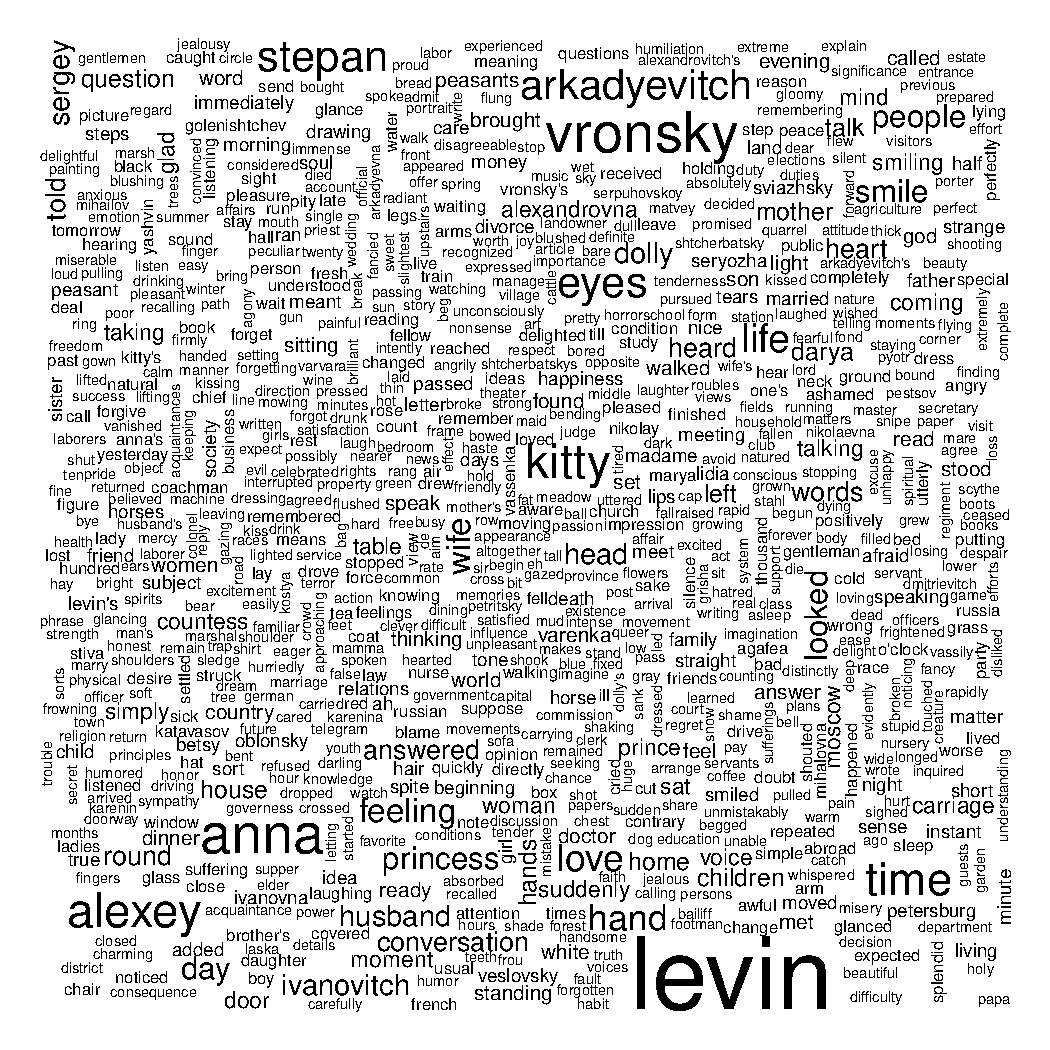
\includegraphics[width=\maxwidth]{figure/unnamed-chunk-8-1} 

\end{knitrout}

\bibliographystyle{apa}
\bibliography{bib}
\nocite{*}
\end{document}
